% Adjust these for the path of the theme and its graphics, relative to this file
%\usepackage{beamerthemeFalmouthGamesAcademy}
\usepackage{../../beamerthemeFalmouthGamesAcademy}
\usepackage{multimedia}
\usepackage{soul}
\usepackage{tikz}
\usepackage{verbatim}
\graphicspath{ {../../} }

% Default language for code listings
\lstset{language=C++,
        morekeywords={each,in,nullptr}
}

% For strikethrough effect
\usepackage[normalem]{ulem}
\usepackage{wasysym}

\usepackage{pdfpages}

% http://www.texample.net/tikz/examples/state-machine/
\usetikzlibrary{arrows,automata}

\newcommand{\modulecode}{COMP260}\newcommand{\moduletitle}{Distributed Systems}\newcommand{\sessionnumber}{5}

\begin{document}
\title{\sessionnumber: \normalsize{Human-Centred Design for AR/VR}}
\subtitle{\modulecode: \moduletitle}

\frame{\titlepage} 
% LEARNING OUTCOMES
\begin{frame}
	\frametitle{Virtual and Augmented Reality Overview:}
	
	\textbf{Learning Outcomes:}
	
	\begin{itemize}
		\item \textbf{Explain} the difference between augmented \& virtual reality. 
		\item \textbf{Discuss} the various forms of haptic feedback.
		\item \textbf{List} and \textbf{describe} the key components that make up the hardware side of reality systems.	
	\end{itemize}
\end{frame}

\begin{frame}
	\frametitle{No One Size Fits All}
	\begin{figure}
		
\includegraphics[scale=.5]{assets/reactivision}
	\end{figure}
\end{frame}

\begin{frame}
	\begin{figure}
		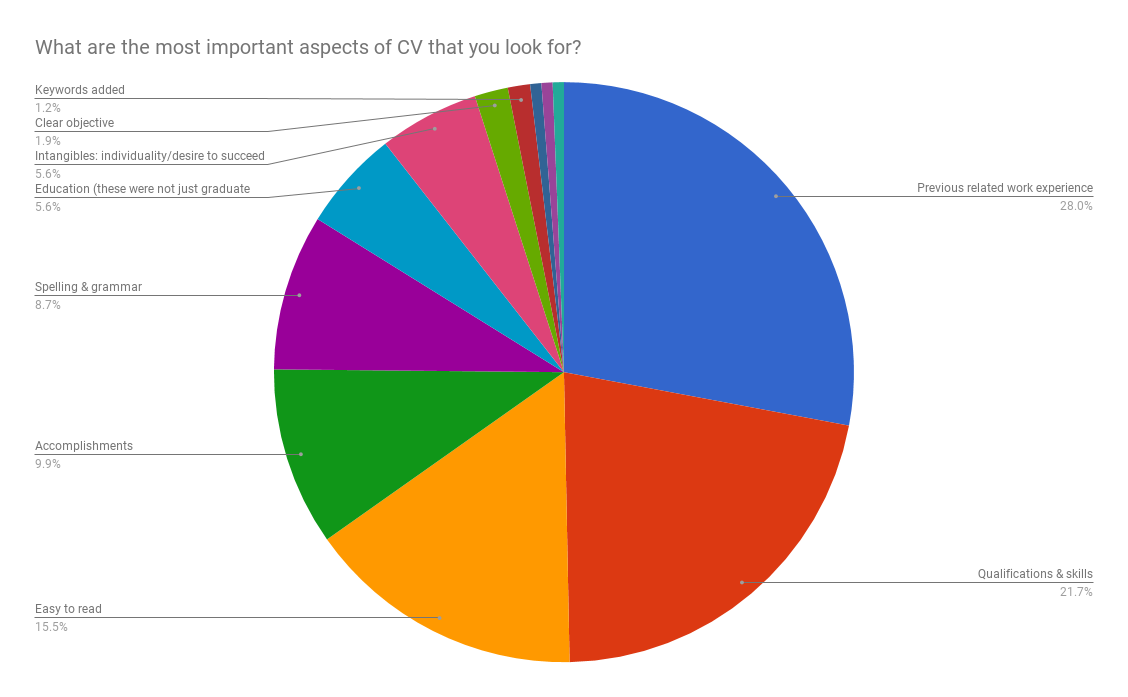
\includegraphics[scale=.27]{assets/priority}
		\caption{2010 Employers Survey}
	\end{figure}
\end{frame}





\end{document}
